\documentclass[11pt]{article}
\usepackage[margin=1in]{geometry}
\usepackage{amsmath,booktabs,graphicx,hyperref}
\hypersetup{hidelinks}
\makeatletter\let\tableinput\@@input\makeatother
\newcommand{\sba}{7(a)}
\title{Do newer loan vintages improve charge-off forecasts? Evidence from SBA portfolios and archived releases}
\author{Yunjie Guo \and Hanqing Yang\thanks{Corresponding author, \texttt{hanqing.yang189@gmail.com}. Affiliation for both authors: Independent Researcher, Suzhou, China.}}
\date{}
\begin{document}
\maketitle
\begin{abstract}
Can recent, incomplete loan vintages improve a five-year portfolio charge-off forecast? We compare the most recent observations at each loan age with a common set of fully mature vintages. In 957,406 US Small Business Administration 7(a) and 504 loan records disbursed in 1999--2015, updating the reference vintages reduces mean absolute error for additive forecasts from 6.44 to 5.16 and from 3.97 to 3.23 percentage points, respectively. The same update raises error for multiplicative development in both programs. A historical upper forecast targeting 90\% nonexceedance is exceeded by all 17 eligible 7(a) vintages whose remaining horizon overlaps the financial crisis. For two subsequent archived issue dates, forecasts scored against a 2025 release favor mature over recent additive increments in each available program--release pair. Rebuilding the December 2022 forecasts from the later file lowers measured error from 0.368 to 0.210 percentage points. The results identify separate risks from the choice of development rule, the slow arrival of calibration outcomes, and revisions to the published loan history.

\end{abstract}
\noindent\textbf{Keywords}\quad small business credit, vintage analysis, charge-offs, forecast evaluation, loss development

\section{Introduction}
A portfolio manager who has observed two years of a loan cohort can see how many loans have already charged off. Forecasting the five-year incidence requires three more years of experience. The last cohort with a complete five-year record is already three years older. For estimating what happens in the ninth quarter of a loan's life, however, the immediately preceding cohort has supplied an observation. Discarding that observation buys a complete historical trajectory at the price of a longer information lag. Using it instead requires an assumption about how well different cohorts can be combined.

This trade-off matters for US Small Business Administration (SBA) portfolios. The Government Accountability Office documents a change in loan performance for borrowers entering the 2007--09 recession and describes the richer economic inputs available to the agency when estimating subsidy costs \cite{gao}. Breeden models the joint role of lifecycle and economic conditions in loan forecasts \cite{breeden}. Patel and Pearce use SBA records to study differences in default risk across borrowers \cite{patel}. Glennon and Nigro model the timing of defaults in SBA lending through survival analysis \cite{glennon}. Ahor evaluates early charge-off rankings across lending regimes and shows the importance of the denominator for unresolved portfolios \cite{ahor}. Our decision is made after disbursement and concerns the future charge-off count of a portfolio. A guarantee purchase, a borrower's first missed payment and a booked charge-off can occur at different times.

Period analysis borrows age-specific experience from a recent calendar window \cite{brenner}. Loss reserving chains successive development factors from incomplete portfolios \cite{mack}. Later insurance filings have been used to test such projections \cite{meyers}, and macroeconomic forecast comparisons can depend on the data edition used to reconstruct an earlier forecast \cite{stark}. These precedents supply the estimators and motivate the archival comparison.

Our empirical contribution is to measure two different changes on the same SBA portfolios. First, at a fixed loan age, how much does replacing mature donor vintages change forecast error when both rules use the same donor weights? We distinguish updating the new charge-off counts from updating the cumulative base of a development factor. Second, holding the final outcomes fixed, does reconstructing the inputs from a later file change which window appears more accurate? A disjoint panel of later disbursements and three archived reference dates indicate how far the initial findings travel. All subsequent extensions were specified after the original results were known. Some later portfolios had already appeared in the archive comparison at other ages.

\section{Sources, cohort and outcome}
We use public SBA Freedom of Information Act records for the \sba{} and 504 programs \cite{sba}. The former provides loan guarantees and the latter finances long-term fixed assets through certified development companies. The archive includes loans still open at the release date. The versioned mirrors preserve agency as-of dates, checked in every record \cite{editions}. The 2020 edition covers both programs from fiscal year 1991. The September 2022 mirror contains \sba{} approvals in fiscal years 2010--19 and 504 approvals from fiscal year 2010 onward \cite{september}. The December 2022 mirror covers \sba{} approvals in fiscal years 1991--2019. The 2025 mirror includes \sba{} approvals in fiscal years 2010--19 and 504 approvals from fiscal year 2010 onward. We score each program separately.

A record enters at its first dated disbursement, within 0--365 days of its dated approval. This rule fixes a maximum gap across the approval-year file boundary. We include loans regardless of later repayment status. The denominator is the number of eligible loan records. A dated charge-off counts if the date lies between disbursement and the snapshot. A status indicating charge-off without a usable event date is tracked as a potentially unlocated event. The additional fraction of such records gives a conservative upper sensitivity for the dated endpoint. A payoff removes the possibility of an ordinary later charge-off, but leaves the loan in the original denominator. Hence all increments below are unconditional event fractions of the funded cohort. Exposure weights, recoveries and realized dollar losses would define different targets. For a contract-term sensitivity, we repeat the forecasts within loans recorded at up to 120 months and above 120 months. The full portfolio also includes missing or nonpositive terms. Term is the value in the file used to form the group. A term recorded after payoff, modification or charge-off may differ from the term available at the landmark. These subgroup results describe the archive and cannot establish prospective segmentation performance.

Write $v$ for the calendar quarter of entry, $j$ for age in quarters, $N_v$ for the cohort count and $x_{vj}$ for dated charge-offs at age $j$ divided by $N_v$. Age one is the disbursement quarter. Thus a 20-quarter outcome measures between approximately 4.75 and 5 years, depending on the disbursement day. Let $F_v(a)=\sum_{j=1}^a x_{vj}$. The primary forecast attaches to quarter end $t=v+a-1$, with $a=8$ and horizon $H=20$. At $t$, age $j$ is visible only for vintages through $t-j+1$. A single-release replay masks later event dates. It cannot recreate the reporting delays or corrections that affected the original historical files. The comparison across archived editions preserves the contents of each file. Its date denotes the snapshot reference date, with public availability following publication.

\section{Forecast construction and evaluation}
For a reference window of $W$ vintages define $A_j(k)=W^{-1}\sum_{i=0}^{W-1}x_{k-i,j}$. The mature-increment forecast adds $\sum_{j=a+1}^H A_j(v+a-H)$ to the observed prefix $F_v(a)$. The period forecast adds $\sum_{j=a+1}^H A_j(v+a-j)$. At each age the latter uses increments from the most recent $W$ calendar quarters visible at issue. Choosing $W=1$ in this formula gives the single-vintage frontier forecast. The primary width is eight. Each reference vintage receives equal weight in additive forecasts.

\paragraph{An information-lag calculation.}
At age $j$, the mean source vintage in the period estimate is younger by $H-j$ quarters than in the mature estimate. For an affine age-specific trajectory $x_{uj}=\alpha_j+\beta_j u$ over the relevant vintages, their difference in projected incidence before clipping is exactly
\[
 \widehat F_{\rm period}-\widehat F_{\rm mature}
     = \sum_{j=a+1}^{H}(H-j)\beta_j .
\]
Indeed averaging an affine function gives its value at the window midpoint, and subtracting cancels the common half-window lag. If the underlying incidence sequence has adjacent differences bounded in magnitude by $b_j$, telescoping gives an absolute difference bounded by $\sum_j (H-j)b_j$. These are statements about the separation of forecasts under stated drift conditions. A reversal after issue can give either forecast the smaller realized error. For $a=8$, all twelve remaining ages contribute to the forecast, with an eleven-quarter freshness gain at age nine and zero gain at age twenty.

\paragraph{Comparators.}
Carry-forward sets the tail to zero. Historical rate takes the average complete incidence of the reference window. The mature development factor multiplies the observed prefix by total charge-offs through $H$ divided by total charge-offs through $a$ in the same complete reference vintages. The age-to-age chain separately computes this pooled count ratio between ages $j-1$ and $j$ using the most recent $W$ vintages observed through $j$, and multiplies the target prefix by the resulting sequence of factors. With a common mature pool $B$ used at every age, the product telescopes:
\[
 \prod_{j=a+1}^{H}\frac{\sum_{u\in B}N_u F_u(j)}
                           {\sum_{u\in B}N_u F_u(j-1)}
  = \frac{\sum_{u\in B}N_u F_u(H)}{\sum_{u\in B}N_u F_u(a)}.
\]
Thus the mature factor and the age-to-age chain form a second within-family comparison of the same choice of information window. This identity requires positive denominators at each step. A denominator of zero leaves the multiplicative forecast undefined. All point estimates are restricted to the interval from the observed prefix to one. The development and chain benchmarks re-scale an early signal from the target portfolio, whereas the additive forecasts transfer later increments directly.

\paragraph{Scoring.}
We average errors equally across quarterly portfolios and report percentage points (pp). A positive signed forecast error denotes overprediction. We separately examine windows from age nine through twenty overlapping 2007Q4--2009Q2, using the NBER recession dates rounded to quarters \cite{nber}. This is a descriptive period comparison. Risk can also change with the composition of disbursements, servicing and recognition practice. A moving-block bootstrap resamples paired errors in contiguous segments with replacement, concatenating and truncating to the original length. We report the central 95\% range of 3,000 resampled mean differences for blocks of eight quarters and assess lengths four and twelve. Shared economic shocks limit the independent replication available from successive cohorts.

\paragraph{Upper forecasts.}
At each issue date, calculate earlier period forecasts using the same landmark and the information observable at each earlier origin. From the last twenty such cohorts whose $H$-quarter outcomes are now known, take the nineteenth smallest value of outcome minus forecast. Add its positive part to the current period estimate and cap at one. Nonexceedance is the fraction of outcomes at or below this upper forecast. Adjacent errors share calendar exposures and can shift together. This rule is a historical calibration diagnostic. A separate scenario scales the projected tail by one-half or two, preserving the observed prefix. It tests sensitivity to late charge-offs without assigning the scenarios probabilities.

\section{Quarterly vintage forecasts}
The 2020 edition supplies 1,615,443 approved \sba{} records and 187,255 approved 504 records. The dated-entry rule retains 1,352,814 and 108,606, respectively, across the full archive. The \sba{} file has 208,215 records missing an entry or approval date and 54,414 outside the entry window. The corresponding 504 counts are 33,114 and 45,535. The main scored vintages run from 1999Q1 through 2015Q4. They contain 883,104 \sba{} and 74,302 504 records across 68 quarters per program. Earlier records train the initial forecasts. The five-year incidence ranges from 2.93\% to 30.23\% in \sba{} and from 0.34\% to 14.94\% in 504. Adding every undated flagged charge-off to the horizon would increase a scored portfolio's incidence by at most 0.011 pp in \sba{} and zero in 504.
\begin{table}[htbp]
\centering\small
\caption{Error at the eight-quarter landmark, percentage points. The overlap column reports mean absolute error (MAE) for portfolios whose remaining observation window intersects 2007Q4--2009Q2. Maximum shortfall is the largest realized incidence minus forecast over all scored vintages.}
\label{tab:accuracy}
\begin{tabular}{lrrrrrr}
\toprule
 & \multicolumn{3}{c}{7(a)} & \multicolumn{3}{c}{504} \\
\cmidrule(lr){2-4}\cmidrule(lr){5-7}
Method & MAE & Overlap & Max. shortfall & MAE & Overlap & Max. shortfall \\
\midrule
\tableinput accuracy.tex
\bottomrule
\end{tabular}
\end{table}
Using the latest available age-specific increments reduces mean absolute error by 1.28 pp in \sba{} and 0.75 pp in 504 (Table~\ref{tab:accuracy}). The period window beats the mature window in 40 and 44 of 68 quarterly comparisons, respectively. The eight-quarter block resampling ranges for period minus mature MAE are $[-3.99,1.09]$ and $[-1.81,0.08]$ pp. In \sba{} the range spans zero for all three block lengths. In 504 its upper endpoint is close to zero for blocks of four and twelve. These ranges summarize sensitivity to which contiguous portfolios are resampled. The blocks span at most twelve quarters and successive forecasts share donors and targets for longer. The ranges cannot quantify uncertainty across independent economic cycles.

The freshness comparison goes the other way for multiplicative development. Allowing new vintages into the successive development factors raises average error by 0.28 pp in \sba{} and 2.24 pp in 504. One 504 chain forecast reaches the 100\% cap. For the 2007Q4 vintage it scales an early incidence of 2.05\% to the cap against a realized 13.00\%. Across leave-one-quarter-out summaries the 504 chain still increases MAE by 1.10 to 2.52 pp relative to the mature factor. Sparse early events can make the product unstable. In \sba{} the mature factor gives the lowest overall MAE, while the single-vintage additive forecast has the lowest MAE in 504. The latter benefits from newer data but also carries greater quarter-specific variation.

The length of the information window matters independently of vintage eligibility. At four and twelve quarters, respectively, period MAE is 4.80 and 5.53 pp for \sba{} and 2.88 and 3.47 pp for 504. Mature increments are less accurate at both widths in both programs. Within short and long term groups, the eight-quarter period window also has lower MAE than mature increments. The reductions are 1.38 and 0.18 pp in \sba{}, and 0.11 and 0.77 pp in 504. Some short-term 504 portfolios lack a nonzero denominator for fitting multiplicative development. All additive forecasts are defined.
\begin{figure}[htbp]
\centering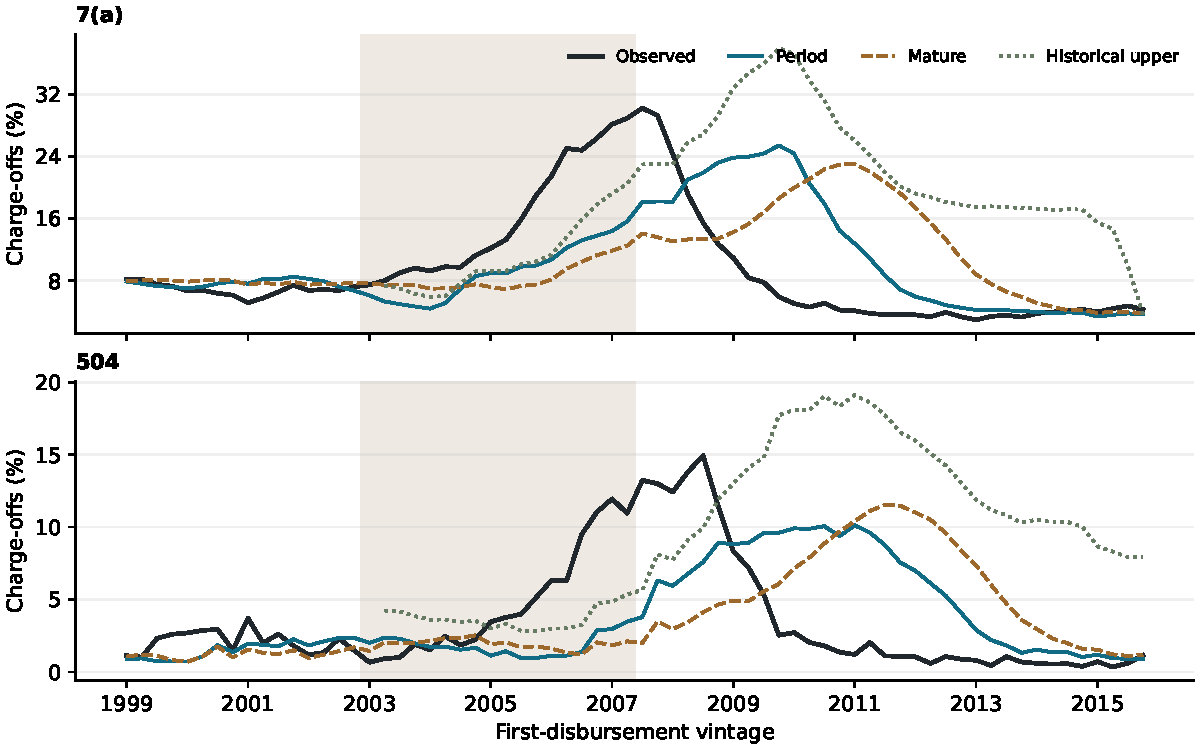
\includegraphics[width=.96\linewidth]{vintages.pdf}
\caption{Dated charge-offs over the first twenty quarters, ordered by disbursement vintage. The shaded vintages have a post-landmark window that overlaps the financial crisis. Each line at a given vintage forecasts the same endpoint from an eight-quarter prefix, except the observed series which uses the mature outcome.}
\label{fig:vintage}
\end{figure}

\subsection{How often did the upper forecasts hold?}
\begin{table}[htbp]
\centering\small
\caption{Historical margins and multiplicative stress scenarios. Covered gives the count below or at the historical upper forecast. Margin and breach are the mean addition above the point forecast and the largest amount above the historical upper forecast, respectively, in pp. Double counts outcomes at or below a doubled tail. Inside counts those between a halved and a doubled tail.}
\label{tab:upper}
\begin{tabular}{llrrrrrr}
\toprule
Program & Window & $n$ & Covered & Margin & Breach & Double & Inside \\
\midrule\tableinput upper.tex
\bottomrule
\end{tabular}
\end{table}
Eighteen vintages per program have a tail that overlaps the financial crisis. Seventeen have the twenty mature forecast errors required to issue the historical upper forecast. In \sba{}, none of these seventeen outcomes falls below or at the upper forecast. The mean addition to the point estimate is only 1.71 pp in that subset, compared with 10.85 pp outside it. Even a doubled forecast tail covers only six of the seventeen outcomes. The 504 upper forecast covers seven of seventeen. These are adjacent vintages exposed to one crisis, so the seventeen misses in \sba{} describe a sustained failure in time.

The error changes direction as older stressed vintages enter the reference set (Figure~\ref{fig:vintage}). For \sba{} disbursements in 2009Q4, the period forecast is 25.42\% against an outcome of 5.90\%. This overprediction and the earlier underpredictions have different implications for a lender estimating future charge-off counts. A mean signed error near zero can coexist with large shortfalls on one side of the cycle. Table~\ref{tab:upper} reports both nonexceedance and the cost of carrying the margin.

\section{Matched weights and a later disbursement panel}

The primary comparison gives equal weight to donor vintages for increments and pools loan counts for the development factors. We repeat both rules with a common weighting convention throughout. For donor cohort $u$ let $w_u$ sum to one within each age-specific pool, using equal weights or weights proportional to the number of funded loans. Write $d_j=\sum_u w_u x_{uj}$ and $b_j=\sum_u w_u F_u(j-1)$. An additive forecast transfers $d_j$ at each remaining age. A multiplicative forecast uses $1+d_j/b_j$. We hold the weighting convention fixed when moving both quantities to recent donors. Every reported comparison uses the same target quarters for the two windows and the two families.

\begin{table}[htbp]
\centering\small
\caption{Recent minus mature MAE (pp) with matched donor weights at age eight. Positive values favor mature donors. The exclusion row retains quarters for which the full donor and target span avoids the financial crisis. Later quarters are disjoint from the original disbursement panel.}
\label{tab:transfer}
\begin{tabular}{llr rrrr}
\toprule
 & & & \multicolumn{2}{c}{Equal vintage weights} & \multicolumn{2}{c}{Loan weights} \\
\cmidrule(lr){4-5}\cmidrule(lr){6-7}
Program & Panel & $n$ & Add & Multiply & Add & Multiply \\
\midrule\tableinput matched.tex
\bottomrule
\end{tabular}
\end{table}

In the full original panel the sign difference across forecast families survives both weighting conventions (Table~\ref{tab:transfer}). Its economic magnitude is sensitive to the years included. At the fixed landmark the earliest donor event that can enter a development factor is in quarter $v-19$ and the last scored event is in $v+19$. Excluding portfolios for which any quarter of that span intersects 2007Q4--2009Q2 leaves 23 quarters in each program. The 7(a) additive advantage of 1.28 pp becomes a disadvantage of 0.04 pp. In 504, the additive advantage shrinks from 0.75 to 0.14 pp. This exclusion also removes the surrounding years and cannot identify a causal recession effect.

Using the September 2025 edition, we score all fifteen subsequent quarterly vintages with complete common coverage (2016Q1--2019Q3), comprising 195,691 \sba{} and 12,477 504 records. We apply the same date mask and age-eight landmark, without tuning a window on these portfolios. With equal donor weights, recent increments improve MAE by 0.15 pp for \sba{} and give up 0.01 pp in 504. Recent development factors increase error in both programs. The 504 file alone supports five further vintages, 2019Q4--2020Q4. There the recent additive window gains 0.26 pp while the two multiplicative forecasts tie on average. We keep these five outside the common comparison.

\paragraph{What changes in a development factor?}
Let $L_{ij}$ denote MAE after choosing the source of increments $i$ and of the cumulative base $j$ separately, each mature ($M$) or recent ($R$). The forecasts retain the original prefix and cap. Following the order-averaged decomposition in Shorrocks \cite{shorrocks}, the increment contribution is $[(L_{RM}-L_{MM})+(L_{RR}-L_{MR})]/2$. Subtracting this from $L_{RR}-L_{MM}$ gives the base contribution. In the original \sba{} panel, with loan weights, the net 0.28 pp increase comprises $+3.22$ pp from updating increments and $-2.94$ pp from updating the cumulative base. In 504 the corresponding terms are $+3.69$ and $-1.46$ pp. The latter portfolio's subsequent common panel gives $-0.02$ and $+0.37$ pp. The hybrid substitutions describe the mechanics of the recorded loss difference. The offset in the historical aggregates does not fix its sign or size elsewhere.

\paragraph{Other US recession windows.}
We use the calendar quarters containing the NBER monthly peak and trough. As before, a target qualifies if any of its twelve remaining quarters overlaps the episode. To preserve the original error history, calibration uses mature errors from the original replay through the 2015Q4 disbursement vintage, then from the later replay. These are retrospective, date-masked errors. Four scored portfolios per program overlap the 2001 downturn but none has twenty mature historical errors, so upper-forecast coverage is unobservable there. For the 2020 downturn (2020Q1--Q2), the historical period upper forecast covers seven of thirteen eligible \sba{} outcomes and ten of thirteen 504 outcomes. In 2007--09 it covered zero and seven of seventeen, respectively. SBA payment relief for eligible outstanding loans during the pandemic changed the setting \cite{relief}. Each count describes one sequence of overlapping portfolios within one macroeconomic episode.

\section{Does reconstructing the archive change the ranking?}
For an early edition $e$ and the 2025 edition $f$, write $\widehat R^{e}$ for the projected additional incidence. The reporting contribution and tail error can be measured separately:
\[
F_v^f(H)-\widehat F_v^e(H)
 = \big[F_v^f(a)-F_v^e(a)\big] +
   \big[F_v^f(H)-F_v^f(a)-\widehat R^e\big].
\]
Rates use the denominator in their respective editions. The first term captures net changes to eligible records and to dates that fall before the cutoff. Opposing revisions can cancel at the portfolio level. In a further check we rebuild the period forecast from the 2025 file, masking all events after the earlier origin. The difference from the archived forecast also captures revisions to the donor histories. Entry support is checked separately for each source and scoring file. The 7(a) final slice ends with FY2019 approvals. We stop at 2019Q3 disbursements to avoid partially observed portfolios. Both September 2022 and September 2025 have continuing 504 files, which also support the later 504 vintages. Donor coverage is complete for all retained targets under the 365-day entry rule.

Define $D_e$ as MAE with the recent window minus MAE with the mature window, calculated using archived inputs and the 2025 outcomes. Define $D_f$ identically after reconstructing both forecasts from the 2025 file with the historical event-date mask. Lower error for recent vintages gives a negative difference. Scoring the identical outcomes at identical ages makes $D_f-D_e$ an input-edition effect on the comparison. For reference, the triangle inequality bounds its magnitude by the mean sum of the absolute revisions in the two forecasts. A gap larger in magnitude than that bound must retain its sign. Individual revisions and bounds are included in the supplement.

\begin{table}[htbp]
\centering\small
\caption{Does the recent window have lower MAE? Differences are recent minus mature MAE in pp, across all supported portfolio ages at each origin. Archived columns use the actual earlier file. Replay columns use date-masked September 2025 inputs. A change in sign reverses the ranking.}
\label{tab:external}
\begin{tabular}{llrr rrrr}
\toprule
 & & & & \multicolumn{2}{c}{Additive} & \multicolumn{2}{c}{Multiplicative} \\
\cmidrule(lr){5-6}\cmidrule(lr){7-8}
As of & Program & Ages & $n$ & Archived & Replay & Archived & Replay \\
\midrule\tableinput external.tex
\bottomrule
\end{tabular}
\end{table}

In the September 2020 \sba{} file, using recent development factors improves MAE by 0.185 pp. Reconstructing the same forecasts from the 2025 file gives the mature factors a 0.215 pp advantage (Table~\ref{tab:external}). The gap moves by 0.400 pp with the scoring outcomes fixed. Two other multiplicative comparisons also change sign, including a 504 gap below 0.01 pp in either direction. The September 2022 504 forecasts give identical archived and reconstructed gaps. These five program--origin pairs share programs, economic conditions and final outcomes. Three reversals are descriptive cases.

\paragraph{Comparison at the primary landmark.}
Only three program--origin pairs support an eight-quarter forecast scored at twenty quarters. In September 2020, the archived additive gap is $-0.010$ pp for \sba{} and $+0.036$ pp for 504. In September 2022 it is $-0.282$ pp for 504. The September 2020 \sba{} gap becomes $+0.066$ pp in the masked replay. Each figure concerns one portfolio. The 2022 \sba{} files cannot supply the later fully represented disbursement quarters required at age eight. Consequently the pooled-age rows in Table~\ref{tab:external} evaluate a mix of remaining horizons and cannot serve as replications of the two-year-landmark result. The two 2022 origins are one quarter apart. Archive as-of dates establish what the files contained. Contemporaneous public access on those exact dates is unverified, which matters especially at a one-quarter remaining horizon.

In the twelve September 2020 \sba{} portfolios, the mean prefix subsequently falls by 0.222 pp while the realized post-landmark increment exceeds its period forecast by 0.116 pp. These components partly offset. The denominator also moves from 161,863 to 162,046 records. In the six December 2022 \sba{} portfolios the mean prefix revision is $-0.112$ pp and mean tail error is $-0.256$ pp. Reconstructing that period forecast from the 2025 edition would report MAE of 0.210 pp in place of 0.368 pp. The aggregate comparison cannot assign the revisions to individual loans.

\section{Interpretation and limits}
There are two distinct ways that more recent observations enter a forecast. An additive estimator replaces older increments with newer unconditional event fractions. A multiplicative estimator also changes the base on which the next growth factor operates. When a cohort has had very few early charge-offs, a sequence of estimated growth factors can propagate a small change in early incidence into a large change in the projected count. Comparing two information windows within each family exposes this difference. The ordering of the two windows in a given historical replay therefore has limited value without the development formula and the individual vintage errors.

Two checks added after the primary comparison address selection and calibration. Retaining all nonnegative approval-to-disbursement delays increases the scored sample to 918,448 \sba{} and 105,171 504 loans. Period versus mature additive MAE is then 5.02 versus 6.26 pp for \sba{} and 3.17 versus 3.99 pp for 504. Moving from the mature development factor to the age-to-age chain still increases MAE in both programs. The period upper forecast again covers zero of seventeen overlapping \sba{} vintages and seven of seventeen 504 vintages. The original entry restriction therefore has a substantial effect on 504 portfolio size while preserving these directional findings.

Keeping the original cohorts and calibrating a separate historical margin for each point forecast changes the picture. During the crisis overlap the mature development factor's upper forecast covers thirteen of seventeen \sba{} outcomes, compared with zero for the period additive center and eleven for the age-to-age chain. In 504 the corresponding counts are eight, seven and eleven. Thus the zero-of-seventeen result is specific to the combination of a period increment forecast and its lagged error margin. Changing the forecast center changes the errors available for calibration as well as the point estimate.

A second operational issue is the lag in feedback. At an eight-quarter landmark the errors used to set the margin come from vintages at least twelve quarters older. The newest errors in a calibration sample can still describe conditions that have passed. This lag is fixed by the outcome horizon even when recent age-specific observations can already influence the point forecast. An archive-based report can make the lag visible by publishing the issue date, most recent mature cohort and largest subsequent breach next to the stated target coverage.

The historical exercise covers one US financial crisis. Adjacent portfolios and the two SBA programs share national economic conditions. The small number of archived issue dates further limits inference about publication revisions in other periods. The upper forecasts measure empirical shortfall risk for a counted portfolio. They have no exchangeability guarantee under a common shock. The public fields identify administrative recognition dates. Changes in collections, accounting and reporting can move them even if underlying borrower distress has a different time path. The entry rule selects relatively prompt disbursements and the analysis gives each loan the same weight. The measured errors apply to these public portfolios. An underwriting, reserve-dollar or macroeconomic capital application would need its own loss definition, exposure weights and validation data.


\paragraph{Data and code.} The replication repository contains aggregate vintage-by-age counts, edition hashes, cohort filters, all scored forecasts, and the executable Python workflow. Each source archive is pinned in the \href{https://github.com/fightforbelief/p16-credit-stress}{replication repository}.
\paragraph{Funding and competing interests.} The authors received no specific funding for this work and declare no competing interests.
\begin{thebibliography}{15}\small\raggedright\setlength{\itemsep}{2pt}
\bibitem{gao} US Government Accountability Office. \emph{Small Business Loans: SBA Generally Incorporated Key Elements for Estimating Subsidy Cost of 7(a) Program}. GAO-20-618, 2020. \url{https://www.gao.gov/products/gao-20-618}.
\bibitem{breeden} J. L. Breeden. Incorporating lifecycle and environment in loan-level forecasts and stress tests. \emph{European Journal of Operational Research} 255 (2016), 649--658. \url{https://doi.org/10.1016/j.ejor.2016.06.008}.
\bibitem{patel} P. C. Patel and J. A. Pearce. Franchisees and loan default on third-party guarantee loans: Evidence from the United States. \emph{Entrepreneurship Theory and Practice} (2020). \url{https://doi.org/10.1177/1042258719853508}.
\bibitem{glennon} D. Glennon and P. Nigro. Measuring the default risk of small business loans: A survival analysis approach. \emph{Journal of Money, Credit and Banking} 37 (2005), 923--947. \url{https://doi.org/10.1353/mcb.2005.0051}.
\bibitem{ahor} I. Ahor. Predicting early default in SBA 7(a) loans: Public-data risk ranking across a regime shift. SSRN working paper, posted 2026. \url{https://doi.org/10.2139/ssrn.7197485}.
\bibitem{brenner} H. Brenner and O. Gefeller. Deriving more up-to-date estimates of long-term patient survival. \emph{Journal of Clinical Epidemiology} 50 (1997), 211--216. \url{https://pubmed.ncbi.nlm.nih.gov/9120515/}.
\bibitem{mack} T. Mack. Distribution-free calculation of the standard error of chain ladder reserve estimates. \emph{ASTIN Bulletin} 23 (1993), 213--225. \url{https://doi.org/10.2143/AST.23.2.2005092}.
\bibitem{meyers} G. Meyers. \emph{Stochastic Loss Reserving Using Bayesian MCMC Models}. 2nd ed., Casualty Actuarial Society, Monograph 8, 2019. \url{https://www.casact.org/sites/default/files/2021-02/08-Meyers.pdf}.
\bibitem{sba} US Small Business Administration, Office of Capital Access. \emph{7(a) and 504 FOIA}. Loan-level data and dictionary. \url{https://data.sba.gov/dataset/7a-504-foia}.
\bibitem{editions} US Small Business Administration. FOIA extracts as of September 30, 2020, December 31, 2022, and September 30, 2025. Version 1 archive mirrors,
\href{https://www.kaggle.com/datasets/thedevastator/sba-loan-guarantee-data-1990-1999}{The Devastator},
\href{https://www.kaggle.com/datasets/williecosta/sba-7a-loan-data}{Willie Costa}, and
\href{https://www.kaggle.com/datasets/kuldeepmishra0496/sba-loan-data}{Kuldeep Mishra}. Archive and member identities are recorded in the replication package.
\bibitem{nber} National Bureau of Economic Research. \emph{US Business Cycle Expansions and Contractions}. \url{https://www.nber.org/research/data/us-business-cycle-expansions-and-contractions}.
\bibitem{stark} T. Stark and D. Croushore. Forecasting with a real-time data set for macroeconomists. Federal Reserve Bank of Philadelphia Working Paper 01-10 (2001). \href{https://www.philadelphiafed.org/the-economy/macroeconomics/forecasting-with-a-real-time-data-set-for-macroeconomists}{Federal Reserve Bank of Philadelphia}.
\bibitem{september} US Small Business Administration. September 30, 2022 FOIA files for 7(a) and 504. Makeover Monday, 2023 week 6. \href{https://github.com/cmcau/makeover_monday_archive/tree/011e5e1e7d19bc8be7eed43c90403dd87c75f8f0/output/2023/w06}{Versioned file archive}.
\bibitem{shorrocks} A. F. Shorrocks. Decomposition procedures for distributional analysis: A unified framework based on the Shapley value. \emph{Journal of Economic Inequality} 11 (2013), 99--126. \url{https://doi.org/10.1007/s10888-011-9214-z}.
\bibitem{relief} US Small Business Administration. COVID-19 resources for small businesses (July 2020). \href{https://www.sba.gov/blog/2020/2020-07/covid-19-resources-small-businesses/}{SBA debt relief description}.
\end{thebibliography}

\end{document}
